\documentclass[12pt,compress,ngerman,utf8,t]{beamer}
\usepackage[ngerman]{babel}
\usepackage{calc}
\usepackage{ragged2e,wasysym,multicol,mathtools}
\usepackage[protrusion=true,expansion=true]{microtype}
\usepackage{booktabs}
\usepackage{multimedia}
\hypersetup{colorlinks=true}

\newcommand{\video}[2]{\movie[width=#2,height=#2,autostart,loop,poster]{}{#1}}

\graphicspath{{images/}}

\title[Vierdimensionale Geometrie]{Die wundersame Welt der \\ vierdimensionalen Geometrie}
\author[Ingo Blechschmidt, Matthias Hutzler]{\scriptsize
\vspace*{-1em} \\
\textbf{Faszination Mathematik/Physik am 5. Juli 2018} \\
\emph{Fragen sind jederzeit willkommen! Bitte nicht bis zum Ende aufsparen.} \\
\medskip
Ingo Blechschmidt und Matthias Hutzler}

%\usetheme{Warsaw}
\useinnertheme[shadow=true]{rounded}
\useoutertheme{split}
\usecolortheme{orchid}
\usecolortheme{whale}
\setbeamerfont{block title}{size={}}

\useinnertheme{rectangles}

\usecolortheme{seahorse}
\definecolor{mypurple}{RGB}{150,0,255}
\setbeamercolor{structure}{fg=mypurple}
\definecolor{myred}{RGB}{150,0,0}
\setbeamercolor*{title}{bg=myred,fg=white}
\setbeamercolor*{titlelike}{bg=myred,fg=white}

\usefonttheme{serif}
\usepackage[T1]{fontenc}
\usepackage{libertine}

\setbeamertemplate{navigation symbols}{}

\setbeamertemplate{title page}[default][colsep=-1bp,rounded=false,shadow=false]
\setbeamertemplate{frametitle}[default][colsep=-2bp,rounded=false,shadow=false,center]

\newcommand{\hil}[1]{{\usebeamercolor[fg]{item}{\textbf{#1}}}}
\setbeamertemplate{frametitle}{%
  \vskip1em%
  \leavevmode%
  \begin{beamercolorbox}[dp=1ex,center]{}%
      \usebeamercolor[fg]{item}{\textbf{\textsf{\Large \insertframetitle}}}
  \end{beamercolorbox}%
}

\setbeamertemplate{footline}{%
  \leavevmode%
  \hfill%
  \begin{beamercolorbox}[ht=2.25ex,dp=1ex,right]{}%
    \usebeamerfont{date in head/foot}
    \insertframenumber\,/\,\inserttotalframenumber\hspace*{1ex}
  \end{beamercolorbox}%
  \vskip0pt%
}

\newcommand{\backupstart}{
  \newcounter{framenumberpreappendix}
  \setcounter{framenumberpreappendix}{\value{framenumber}}
}
\newcommand{\backupend}{
  \addtocounter{framenumberpreappendix}{-\value{framenumber}}
  \addtocounter{framenumber}{\value{framenumberpreappendix}}
}

\begin{document}

\frame{
  \centering
  \includegraphics[width=0.4\textwidth]{great-grand-120-cell}
  \smallskip

  \titlepage
}


\section{Grundlagen}

\begin{frame}[plain,c]
  \centering
  \Large
  \hil{Wie geht's weiter?}

  1, \pause $\infty$, \pause 5, \pause 6, \pause \hil{??}
\end{frame}
\addtocounter{framenumber}{-1}


\subsection{Vier Dimension: was ist das?}

\begin{frame}{Vier Dimensionen?}
  \centering
  \only<1>{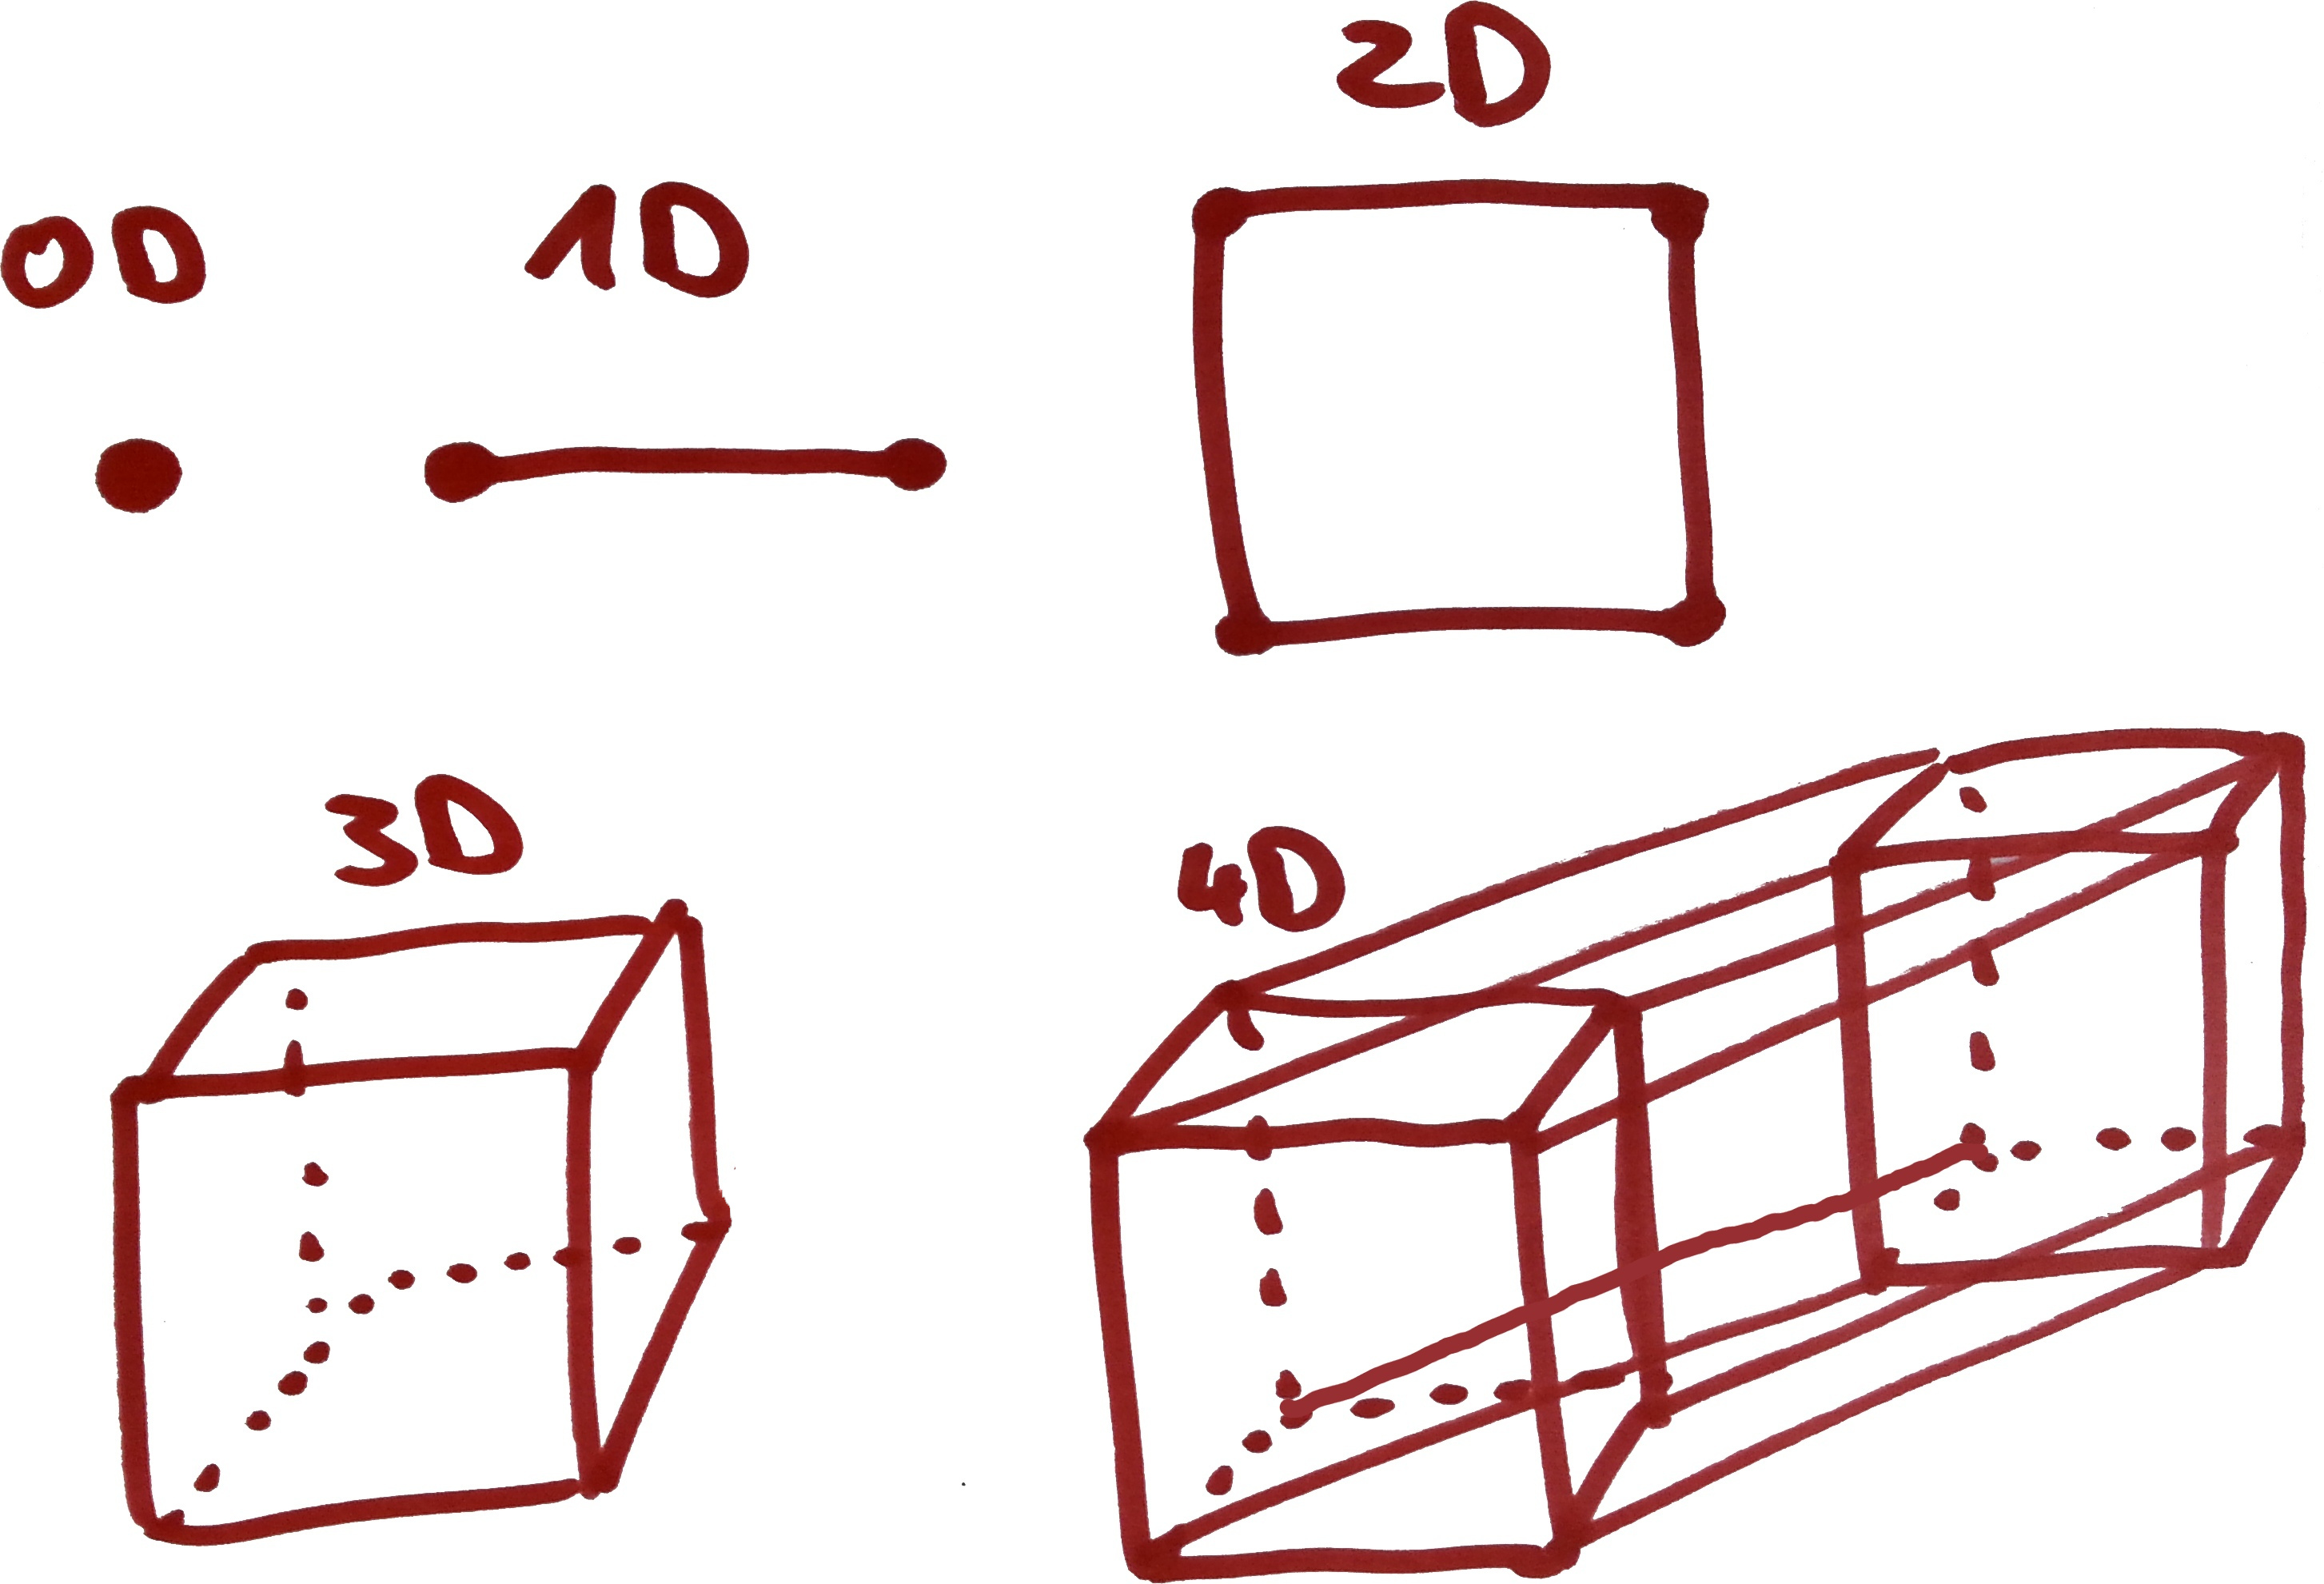
\includegraphics[width=0.9\textwidth]{4d-tesseract}}
  \only<2>{\includegraphics[width=0.9\textwidth]{4d-pentachoron}}
  \only<3>{\includegraphics[width=0.9\textwidth]{prisoner}}
  \par
  % Skizze Punkt, Linie, Quadrat, Würfel, nach \pause Tesserakt
  % Skizze Punkt, Linie, Dreieck, Tetraeder, 4-dimensionales Simplex
  % Sache mit Projektion erklären
  % klarstellen, dass wir über vierdimensionalen Raum (nicht Raum+Zeit) sprechen
  % nicht: 11-dimensionaler Quantenschaum
  % Wo erkennt man die drei Dimensionen in der realen Welt?
  % Gefängnisse (Quadrat genügt im Flachland, Würfel genügt in 3D, genügt nicht in 4D)
\end{frame}


\section[Schnitte]{Schnitttheorie}

\subsection{Ankunft eines Hyperballs}

\begin{frame}{Ankunft eines Hyperballs}
  \centering
  \includegraphics[width=0.9\textwidth]{a-hyperball-arrives}
  \par
\end{frame}


\subsection[und eines Tesserakts]{Ankunft eines Tesserakts}

\begin{frame}{Ankunft eines Tesserakts}
  \centering
  \includegraphics[width=0.9\textwidth]{a-tesseract-arrives}
  \par
\end{frame}

% Jetzt Ecken & Co. zählen


\subsection{Knotentheorie}

\begin{frame}{Schnürsenkel binden}
  % Erklären, dass Schnürsenkel immer aufgehen würden
  \centering
  \includegraphics[width=0.65\textwidth]{trefoil-knot}
  \par
\end{frame}

%Verhedderbar
%in 3D: Schnur, Schnur; 2, 2; 1, 1
%in 3D: Punkt, Fläche;  0, 1; 0, 2
%in 2D: Schnur, Punkt;  1, 2; 1, 0
%in 4D: Schnur, Fläche; 3, 2; 1, 2
%
%Beh.: Dimensionen addiert muss >= n - 1 sein, damit Verhedderung möglich ist
%
%Nicht verhedderbar
%in 3D: Punkt, Schnur; 3, 2; 0, 1
%in 3D: Punkt, Punkt;  3, 3; 0, 0
%in 4D: Punkt, Fläche      ; 0, 2
%in 4D: Schnur, Schnur     ; 1, 1


\section[Größen]{Größen in vier Dimensionen}

\subsection{Volumenverhältnisse}

\begin{frame}{Hypervolumen von Hyperkugeln}
  \centering
  \vspace*{-0.5em}
  \includegraphics[width=0.4\textwidth]{sizes-1}
  \bigskip
  % vorher gscheite Definition der Hyperkugel
  % Bild vom Kreis im Quadrat
  % Bild vom Zylinder im Würfel
  % Bild von der Kugel im Würfel

  \small
  \begin{tabular}{lll}
    \toprule
    Dimension & Hypervolumen & \\\midrule
    $n = 2$ & $\pi / 4$ & $\approx 0{,}785 \,\mathrm{m}^2$ \\
    $n = 3$ & $\pi / 6$ & $\approx 0{,}524 \,\mathrm{m}^3$ \\
    $n = 4$ & $\pi^2 / 32$ & $\approx 0{,}308 \,\mathrm{m}^4$ \\
    $n = 5$ & $\pi^2 / 60$ & $\approx 0{,}164 \,\mathrm{m}^5$ \\
    $n = 6$ & $\pi^3 / 384$ & $\approx 0{,}081 \,\mathrm{m}^6$ \\
    $n = 7$ & $\pi^3 / 840$ & $\approx 0{,}037 \,\mathrm{m}^7$ \\
    $n \to \infty$ & $\to 0$ \\
    \bottomrule
  \end{tabular}\par
\end{frame}


\subsection{Küssende Hyperkugeln}

\begin{frame}[plain,c]
  \centering\Huge
  \scalebox{2.6}{\hil{Liebe ist}} \\[0.6em]
  \scalebox{2.6}{\hil{wichtig.}}

  \bigskip
  \bigskip

  \scalebox{2.6}{\hil{$\boldsymbol{\heartsuit}$}}
  \par
\end{frame}
\addtocounter{framenumber}{-1}


\begin{frame}{Küssende Hyperkugeln}
  % Bild vier Kreise an den Ecken des Zweiheitsquadrats und Kreis in der Mitte
  \centering
  \vspace*{-1em}
  \includegraphics[width=0.3\textwidth]{sizes-2}
  \bigskip

  {\small
  \begin{tabular}{lll}
    \toprule
    Dimension & Radius der inneren Hyperkugel & \\\midrule
    $n = 2$ & \pause $\sqrt{2} - 1$ \\
    \pause
    $n = 3$ & \pause $\sqrt{3} - 1$ \\
    \pause
    $n = 4$ & $\sqrt{4} - 1$ \\
    \pause
    $n$ & $\sqrt{n} - 1$ \\
    \bottomrule
  \end{tabular}\par}
  \bigskip

  \centering
  \hil{Die Entfernung zu den Ecken wird immer größer.}
  \par
\end{frame}


\subsection[Relativität]{Allgemeine Relativitätstheorie}

\begin{frame}{Allgemeine Relativitätstheorie}
  \vspace*{-1em}
  \begin{center}
    \includegraphics[height=0.3\textheight]{einstein}
    \qquad
    \includegraphics[height=0.3\textheight]{gravitational-waves}
  \end{center}

  Einsteins gefeierte \hil{Feldgleichung} besagt
  \[ G = \kappa \cdot T, \]
  wobei
  \begin{itemize}
    \item $G$ die \hil{Raumkrümmung} angibt,
    \item $T$ die \hil{Massenverteilung} misst und
    \item $\kappa$ eine Konstante ist.
  \end{itemize}

  In $2+1$ Dimensionen impliziert die Gleichung~$T = 0$.
  Nur in vier und mehr Dimensionen ist die Theorie nichttrivial.
\end{frame}



\section{Platonische Körper}

\newcommand{\solid}[5]{\begin{column}{0.31\textwidth}\centering\hil{#2}\par#5E, #4K, #3F\\\medskip\includegraphics[height=0.7\textwidth]{#1}\end{column}}
\newcommand{\solidd}[3]{\begin{column}{0.4\textwidth}\centering\hil{#2}\par#3\\\medskip\includegraphics[height=1.9cm]{#1}\end{column}}
\newcommand{\solidde}[3]{\begin{column}{0.33\textwidth}\centering\hil{#2}\par{\scriptsize#3\\}\medskip\includegraphics[height=1.9cm]{#1}\end{column}}
\newcommand{\solidv}[1]{\begin{column}{0.3\textwidth}\centering\hil{$\phantom{A}$}\par$\phantom{A}$\\\medskip\video{images/#1.mp4}{1.9cm}\end{column}}


\subsection{In 3d}

\begin{frame}{Platonische Körper in 3d}
  \begin{columns}[c]
    \solid{tetrahedron}{Tetraeder}{4}{6}{4}
    \solid{hexahedron}{Hexaeder}{6}{12}{8}
    \solid{octahedron}{Oktaeder}{8}{12}{6}
  \end{columns}
  \bigskip
  \begin{columns}[c]
    \solid{dodecahedron}{Dodekaeder}{12}{30}{20}
    \solid{icosahedron}{Ikosaeder}{20}{30}{12}
  \end{columns}
\end{frame}


\subsection{In 4d}

\begin{frame}{Platonische Körper in 4d}
  \only<1>{
    \begin{columns}[c]
      \solidd{tetrahedron}{Tetraeder}{4E, 6K, 4F}
      \solidd{005-cell}{Pentachoron}{5E, 10K, 10F, 5Z}
      \solidv{005-cell}
    \end{columns}
  }

  \only<2>{
    \begin{columns}[c]
      \solidd{hexahedron}{Hexaeder}{8E, 12K, 6F}
      \solidd{008-cell}{Octachoron}{16E, 32K, 24F, 8Z}
      \solidv{008-cell}
    \end{columns}
    \vspace*{2em}
    \begin{columns}[c]
      \solidd{octahedron}{Oktaeder}{6K, 12K, 8F}
      \solidd{016-cell}{Hexadecachoron}{8E, 24K, 32F, 16Z}
      \solidv{016-cell}
    \end{columns}
  }

  \only<3>{
    \begin{columns}[c]
      \solidd{dodecahedron}{Dodekaeder}{20E, 30K, 12F}
      \solidd{120-cell}{Hecatonicosachoron}{600E, 1200K, 720F, 120Z}
      \solidv{120-cell}
    \end{columns}
    \vspace*{2em}
    \begin{columns}[c]
      \solidd{icosahedron}{Ikosaeder}{12E, 30K, 20F}
      \solidd{600-cell}{Hexacosichoron}{120E, 720K, 1200F, 600Z}
      \solidv{600-cell}
    \end{columns}
  }

  \only<4>{
    \centering
    \hil{Icositetrachoron}\par
    24E, 96K, 96F, 24Z\\\medskip\bigskip
    \includegraphics[width=0.4\textwidth]{024-cell} \qquad
    \video{images/024-cell.mp4}{0.4\textwidth}
  }
\end{frame}

\begin{frame}{Pflasterungen}
  \centering
  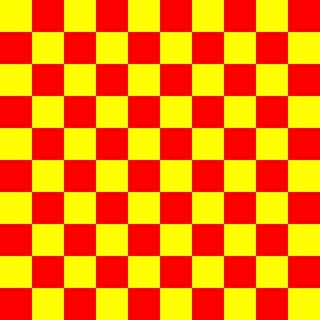
\includegraphics[height=0.6\textheight]{tesselation-squares}
  \qquad
  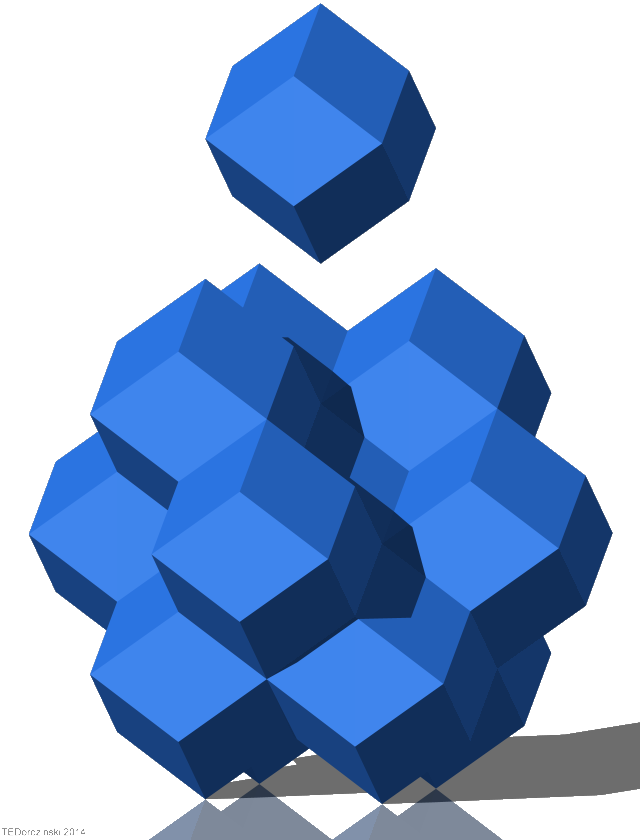
\includegraphics[height=0.6\textheight]{hyperdiamond-3d}
  \bigskip

  \hil{Der 24-Zeller pflastert den vierdimensionalen Raum.}
\end{frame}


\subsection{Ausblick}

\begin{frame}{Die vierte Dimension \ldots}
  \begin{enumerate}
    \item ist faszinierend schön,

    \item hilft beim Verständnis der dritten Dimension,

    \begin{center}
      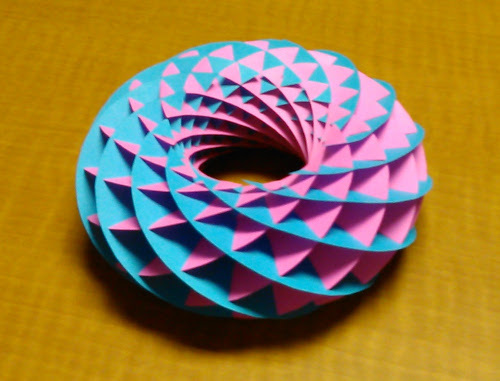
\includegraphics[height=0.3\textheight]{torus-circles}
      \qquad\qquad
      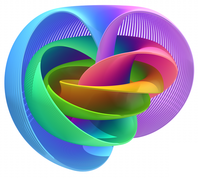
\includegraphics[height=0.3\textheight]{hopf-fibration}
    \end{center}

    \item ist unabdingbar für die moderne Physik und

    \item ist als einzige Dimension noch größtenteils unverstanden.

    \begin{center}
      \begin{tabular}{l|rrrrrrrrrr}
        Dimension & 1 & 2 & 3 & 4 & 5 & 6 & 7 & 8 & 9 & \ldots \\
        Anzahl Sphären & 1 & 1 & 1 & \hil{??} & 1 & 1 & 28 & 2 & 8 & \ldots
      \end{tabular}
    \end{center}
  \end{enumerate}
\end{frame}

\begin{frame}[plain,c]
  \centering
  \begin{columns}
    \begin{column}{0.4\textwidth}
      \centering
      \hil{Catharina Stroppel} \\
      $\phantom{\text{g}}$Knotentheoretikerin$\phantom{\text{g}}$ \\
      \smallskip
      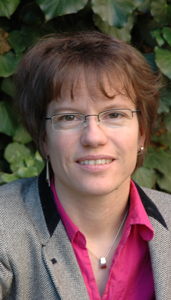
\includegraphics[height=0.5\textheight]{catharina-stroppel}
    \end{column}
    \begin{column}{0.6\textwidth}
      \centering
      \hil{Julia Grigsby} \\
      niedrigdimensionale Topologin \\
      \smallskip
      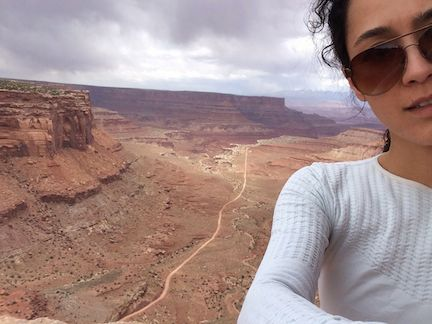
\includegraphics[height=0.5\textheight]{julia-grigsby}
    \end{column}
  \end{columns}
\end{frame}


\section[4d-Labyrinth]{Ein vierdimensionales Labyrinth}

\begin{frame}{Ein vierdimensionales Labyrinth}
  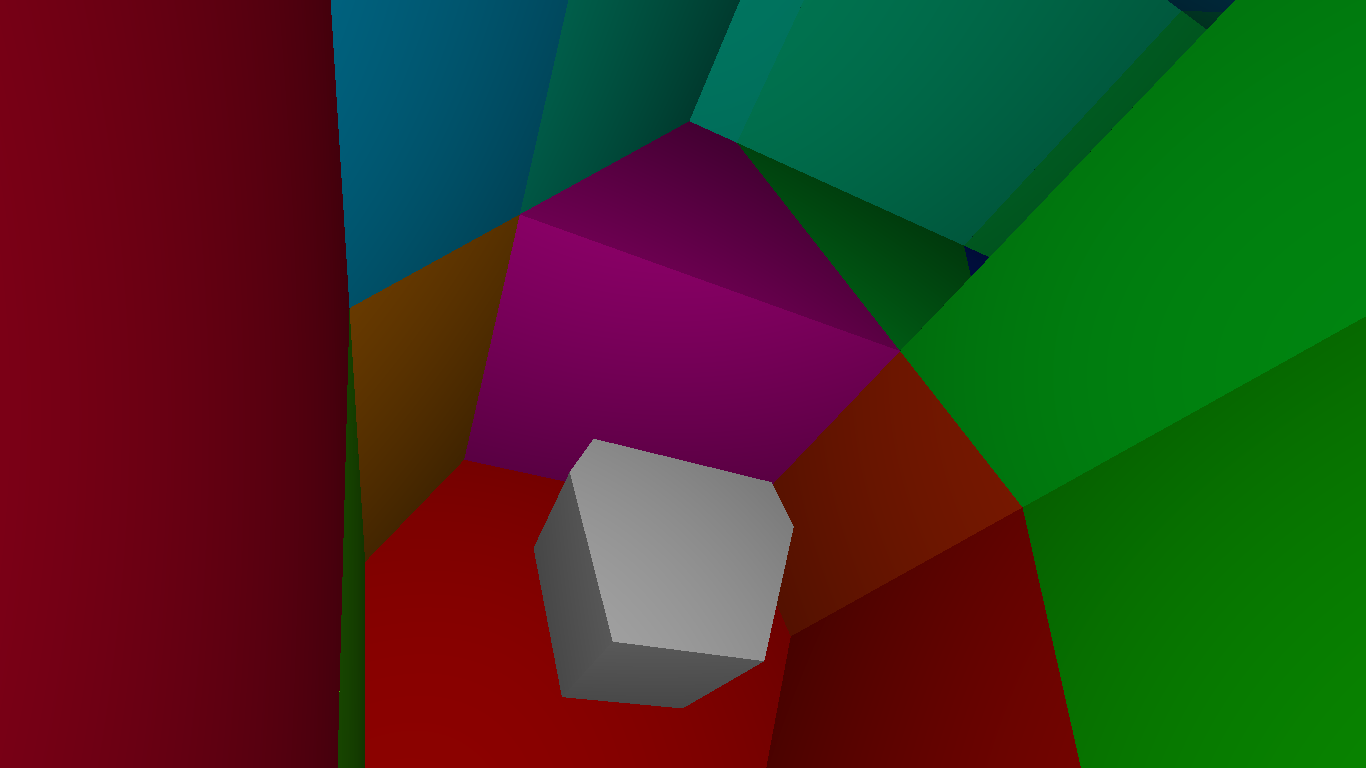
\includegraphics[width=\textwidth]{4d-labyrinth}
\end{frame}


\backupstart
\appendix

\section{Bildquellen}

\begin{frame}{Bildquellen}
  \tiny

  \only<1>{Bilder vier-dimensionaler Körper von Robert Webb, mit seiner
  \emph{Stella}-Software erzeugt: \\
  \url{https://en.wikipedia.org/wiki/File:Ortho_solid_011-uniform_polychoron_53p-t0.png} \\
  \url{https://en.wikipedia.org/wiki/File:Schlegel_wireframe_5-cell.png} \\
  \url{https://en.wikipedia.org/wiki/File:Schlegel_wireframe_8-cell.png} \\
  \url{https://en.wikipedia.org/wiki/File:Schlegel_wireframe_16-cell.png} \\
  \url{https://en.wikipedia.org/wiki/File:Schlegel_wireframe_24-cell.png} \\
  \url{https://en.wikipedia.org/wiki/File:Schlegel_wireframe_120-cell.png} \\
  \url{https://en.wikipedia.org/wiki/File:Schlegel_wireframe_600-cell_vertex-centered.png}}

  \only<2>{Verschiedene Bilder: \\
  \url{http://4.bp.blogspot.com/_TbkIC-eqFNM/S-dK9dd1cUI/AAAAAAAAFjA/d8qdTHhKy1U/s320/tesseract+unfolded.png} \\
  \url{http://gwydir.demon.co.uk/jo/tess/optical6.gif}
  \url{https://commons.wikimedia.org/wiki/File:Blue_Trefoil_Knot.png} \\
  \url{https://en.wikipedia.org/wiki/File:Dodecahedron.svg} \\
  \url{https://en.wikipedia.org/wiki/File:Hexahedron.svg} \\
  \url{https://en.wikipedia.org/wiki/File:Icosahedron.svg} \\
  \url{https://en.wikipedia.org/wiki/File:Octahedron.svg} \\
  \url{https://en.wikipedia.org/wiki/File:Tetrahedron.svg} \\
  \url{https://mathlesstraveled.files.wordpress.com/2017/01/villarceau-torus-small.jpg} \\
  \url{https://upload.wikimedia.org/wikipedia/commons/1/1e/600-cell.gif} \\
  \url{https://upload.wikimedia.org/wikipedia/commons/2/24/HC_R1.png} \\
  \url{https://upload.wikimedia.org/wikipedia/commons/7/72/Rhombic_dodecahedra_b.png} \\
  \url{https://upload.wikimedia.org/wikipedia/commons/a/a0/16-cell.gif} \\
  \url{https://upload.wikimedia.org/wikipedia/commons/c/cf/Hexahedron_flat_color.svg} \\
  \url{https://upload.wikimedia.org/wikipedia/commons/d/d6/8-cell-orig.gif} \\
  \url{https://upload.wikimedia.org/wikipedia/commons/d/d8/5-cell.gif} \\
  \url{https://upload.wikimedia.org/wikipedia/commons/f/f4/24-cell.gif} \\
  \url{https://upload.wikimedia.org/wikipedia/commons/f/f9/120-cell.gif} \\
  \url{https://upload.wikimedia.org/wikipedia/commons/thumb/b/b9/Hopf_Fibration.png/250px-Hopf_Fibration.png} \\
  \url{https://upload.wikimedia.org/wikipedia/en/0/09/Dali_Crucifixion_hypercube.jpg} \\
  \url{https://www2.bc.edu/julia-grigsby/Eli_Moab_6in.JPG} \\
  \url{http://www.gnuplotting.org/figs/klein_bottle.png} \\
  \url{http://www.math.uni-bonn.de/ag/stroppel/Picture_cs2.jpg}}
\end{frame}



\subsection{Ein 4d Fraktal}

\begin{frame}{Ein vierdimensionales Fraktal}
  \justifying
  Ihr kennt das Mandelbrotfraktal.
  Vielleicht kennt ihr auch die Juliafraktale, von denen es je eins für jeden
  Punkt der Ebene gibt.
  Aber wusstet ihr, dass diese unendlich vielen Fraktale nur zweidimensionale
  Schnitte eines vereinheitlichten vierdimensionalen Fraktals ist?
  Wir laden euch ein,
  \href{https://rawgit.com/MatthiasHu/FractalsWebGL/4d/page.html}{damit zu spielen}.
  \bigskip

  \centering
  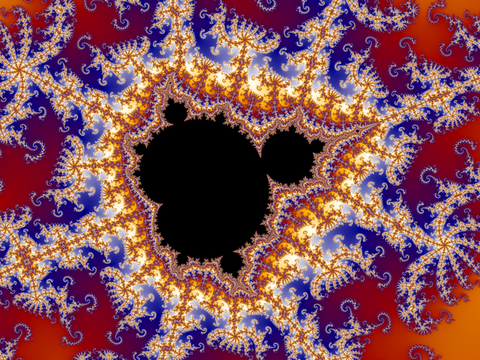
\includegraphics[width=0.5\textwidth]{mandelbrot}
  \par
\end{frame}


\subsection{In beliebigen Dimensionen}

\begin{frame}{In beliebigen Dimensionen}
  \centering
  \begin{tabular}{ll}
    \toprule
    Dimension & Anzahl platonischer Körper \\ \midrule
    $n = 1$ & 1 (nur die Linie) \\
    $n = 2$ & $\infty$ (Dreieck, Quadrat, Fünfeck, Sechseck, \ldots) \\
    $n = 3$ & 5 \\
    $n = 4$ & 6 \\
    $n = 5$ & 3 (nur Simplex, Hyperwürfel und sein Duales) \\
    $n = 6$ & 3 (nur Simplex, Hyperwürfel und sein Duales) \\
    $n = 7$ & 3 (nur Simplex, Hyperwürfel und sein Duales) \\
    $n = 8$ & 3 (nur Simplex, Hyperwürfel und sein Duales) \\
    \emph{und so weiter} \\
    \bottomrule
  \end{tabular}
  \par
\end{frame}


\subsection[Verkleben]{Zusammenkleben vierdimensionaler Formen}

\begin{frame}{Übersicht}
  \begin{columns}[c]
    \solidde{005-cell}{Pentachoron}{5E, 10K, 10F, 5Z}
    \solidde{008-cell}{Octachoron}{16E, 32K, 24F, 8Z}
    \solidde{016-cell}{Hexadecachoron}{8E, 24K, 32F, 16Z}
  \end{columns}
  \bigskip
  \bigskip
  \begin{columns}[c]
    \solidde{120-cell}{Hecatonicosachoron}{600E, 1200K, 720F, 120Z}
    \solidde{600-cell}{Hexacosichoron}{120E, 720K, 1200F, 600Z}
    \solidde{024-cell}{Icositetrachoron}{24E, 96K, 96F, 24Z}
  \end{columns}
\end{frame}

\begin{frame}{Kleben vierdimensionaler Formen}
  \centering
  \begin{columns}
    \begin{column}{0.3\textwidth}
      \centering
      \hil{Würfel} \\
      \smallskip
      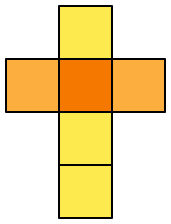
\includegraphics[height=0.35\textheight]{cube-net}
    \end{column}
    \begin{column}{0.3\textwidth}
      \centering
      \hil{Tesserakt} \\
      \smallskip
      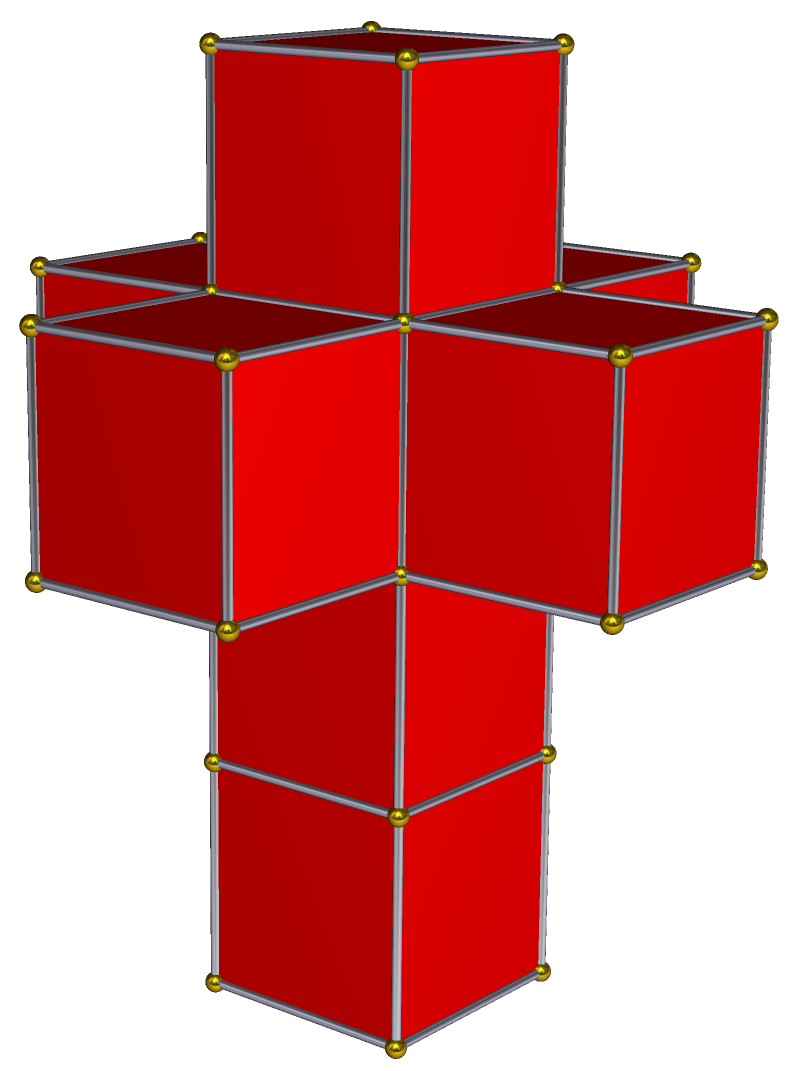
\includegraphics[height=0.35\textheight]{008-cell-net}
    \end{column}
  \end{columns}
  \bigskip
  \bigskip

  \begin{columns}
    \begin{column}{0.3\textwidth}
      \centering
      \hil{16-Zeller} \\
      \smallskip
      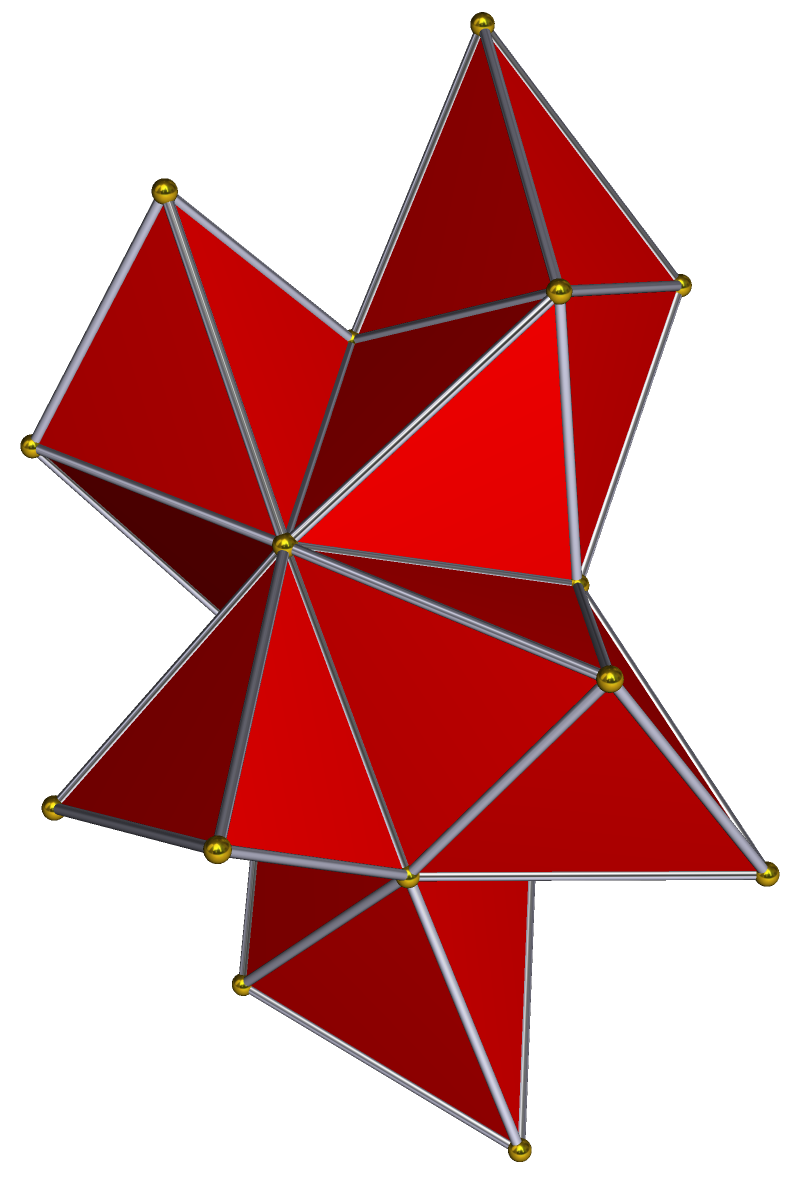
\includegraphics[height=0.3\textheight]{016-cell-net}
    \end{column}
    \begin{column}{0.3\textwidth}
      \centering
      \hil{24-Zeller} \\
      \smallskip
      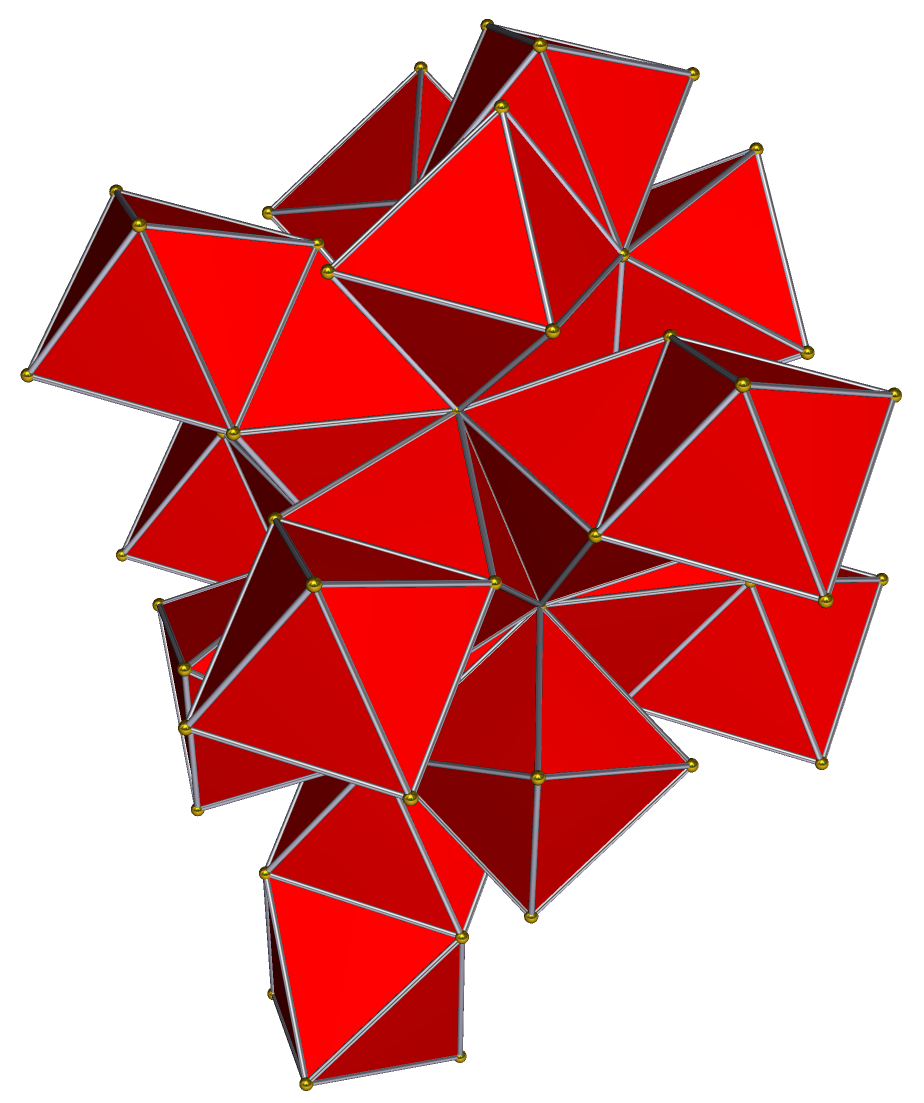
\includegraphics[height=0.3\textheight]{024-cell-net}
    \end{column}
  \end{columns}
\end{frame}

\begin{frame}[plain]
  \centering
  \medskip
  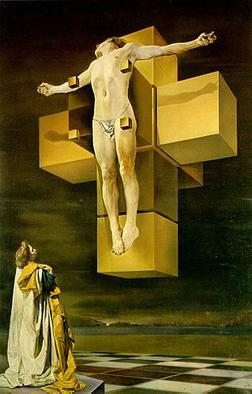
\includegraphics[height=0.95\textheight]{salvador-dali} \\
  \scriptsize
  Salvador Dalí: \hil{Corpus Hypercubus} (1954)
\end{frame}

\backupend

\end{document}


Ecken:     2 4  8 16
Kanten:    1 4 12 32    32 = (16 * 4) / 2    12 = (8 * 3) / 2
Flächen:   0 1  6 24    (3über2)*8/4 = 6     (4über2)*16/4 = 24 = 2^2 * (4über2)
Volumina:  0 0  1  8
4-Vol.:    0 0  0  1

* Raumzeit in 2+1 Dimensionen ist schlecht wegen: Feldgleichung hat zu wenig
  Unbekannte. Masse müsste immer Null sein. (?)
* Kommutativität von gewissen Rotationen; Verknüpfungen von Rotationen ist nicht
  unbedingt Rotation (einer Ebene)! (?)
* (Rotationen nicht um Achsen, sondern "um Ebenen"; besser: Man rotiert immer "in
  einer Ebene".)
* Quaternionen?
* Ist jedes Element der SO(4) eine Rotation einer Ebene? Nein. (-Id)
* Ist jedes Element der SO(4) Verknüpfung zweier Spiegelungen an Hyperebenen? Nein.

Man könnte den Vortrag auch mit dem bekannten Witz (Mathematikerin, Physikerin,
Konferenz, Schwierigkeit, ganz einfach: dann n gegen 11) beginnen. Und dann
gleich dazu sagen, dass es bei uns um räumliche Dimensionen geht.
